\chapter{Related Works}

\section{Image Style Transfer}
 Gatys \textit{et al}. \cite{Gatys_2016_CVPR} introduced \textit{A Neural Algorithm 
of Artistic Style} which enables the creation of novel images that seamlessly blend 
the subject matter of a photograph with the artistic style of a famous artwork.
In rendering the semantic content of an image in various styles, the problem was
the lack of effective image representations that can explicitly encode semantic 
information and separate image content and style. 
\textit{A Neural Algorithm of Artistic Style} \cite{Gatys_2016_CVPR} is able to 
analyze the visual characteristics of an image and separate them into two distinct 
components: the content and the style.
The content refers to the subject or object depicted in the image, while the style 
refers to the visual techniques manifested in a painting, such as touch and mood.

The algorithm in the paper uses a convolutional neural network (CNN) to extract
content and style features from two input images. The goal is to generate an 
output image that minimizes the difference between the content and style features 
of the input and output images, as measured by two loss functions defined in the 
paper. 

To minimize the difference in content features between the input and output images,
it is necessary to consider reducing the content loss function. 
Let $\vec{p}$ and $\vec{x}$ be the input image and the image that is generated by
the model, and  $P^l$ and $F^l$ be their feature representations of these images in 
layer l of the CNN. Then the loss function of the content of images is defined as:

\begin{equation}
    \label{contentloss}
    \mathcal{ L}_{content}(\vec{p}, \vec{x}, l)=\frac{1}{2} \sum_{i, j}\left(F_{i j}^l-P_{i j}^l\right)^2
\end{equation}
Similarly, to minimize the difference in style features between the input and
output images, we consider reducing the style loss function. The style of an 
image can be represented by the correlations of the outputs of the filters in 
each layer. This feature correlation is given by a Gram matrix, which is 
expressed as:
\begin{equation}
    G_{i j}^l = \sum_k F_{i k}^l F_{j k}^l 
\end{equation}
Let $\vec{a}$ and $\vec{x}$ be the input image and the image that is generated by
the model, and $A^l$ and $G^l$ be their style representations of these images in 
kayer l of the CNN. The contribution of layer l to the total loss can be 
expressed as:
\begin{equation}
    E_l=\frac{1}{4 N_l^2 M_l^2} \sum_{i, j}\left(G_{i j}^l-A_{i j}^l\right)^2
\end{equation}
Based on this, we can define the loss function for the style of images as:
\begin{equation}
    \label{styleloss}
    \mathcal{ L}_{style}(\vec{a}, \vec{x})=\sum_{l=0}^\mathcal{ L}w_{l}E_{l}
\end{equation}
To transfer the style of image $\vec{a}$ to image $\vec{p}$, it is needed to 
create a new image that maintains the content representation of $\vec{p}$ 
while adopting the style representation of $\vec{a}$. To achieve this, we must 
minimize both Equation \ref{contentloss} and Equations \ref{styleloss}.
The final loss function to minimize is:

\begin{equation}
    \mathcal{ L}_{total}(\vec{p}, \vec{a}, \vec{x})=\alpha\mathcal{ L}_{content}(\vec{p}, \vec{x})+\beta\mathcal{ L}_{style}(\vec{a}, \vec{x})
\end{equation}


Figure \ref{output_IST} shows the images generated using this algorithm.
絵の出所の説明。

筆のタッチなどのスタイルが適応されていて、良い結果だと思う。が、色味や
特徴的なオブジェクトのトランスファーが行われてしまっている。
私が取り組むものではそれはやりたくない。

\begin{figure}
    \centering
    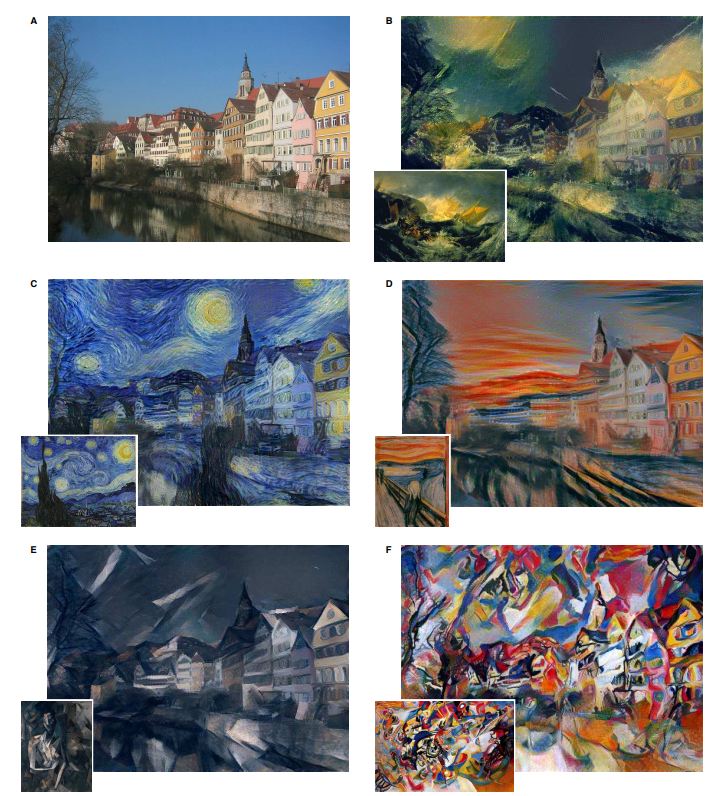
\includegraphics[width=150truemm]{resources/3_related_work/outputs_IST.png}
    \caption{
      なにかかく. Figure taken from
      \cite{Gatys_2016_CVPR}. 
    }
    \label{output_IST}
\end{figure}
\clearpage

\section{強化学習版}
Learn to paint \cite{Huang_2019_ICCV} 
\section{Learn to PaintのCNN版}
Paint Transformers \cite{liu2021paint}

その論文にて課題として残っている点は何であるか、自分の研究はそれとはどのように異なるか、という点が明確になるように